\section{Formalizing Novelty} 

\abovedisplayskip=4pt plus 2pt minus 1pt 
\abovedisplayshortskip=2pt plus 1pt minus 1pt 
\belowdisplayskip=4pt plus 2pt minus 1pt 
\belowdisplayshortskip=2pt plus 1pt minus 1pt


We present frameworks for formalizing novelty for static or learning-based agents, operating in a setting where handling unknown items is required.  Fig.~\ref{fig:elements} shows the main elements of a novelty problem for task $\cal T$. 
 The formulation can support a wide range of novelty problems including being robust to novelties, detecting novelties, learning from novelties or generating novelties.   
 The paper's formalization is about theories, rather than ``a theory,'' because when the definition's set of items and associated functions are provided, a different theory of novelty is defined.  There are infinitely many such theories of novelty for any given task.





 
\begin{figure}[t]
 \centering
    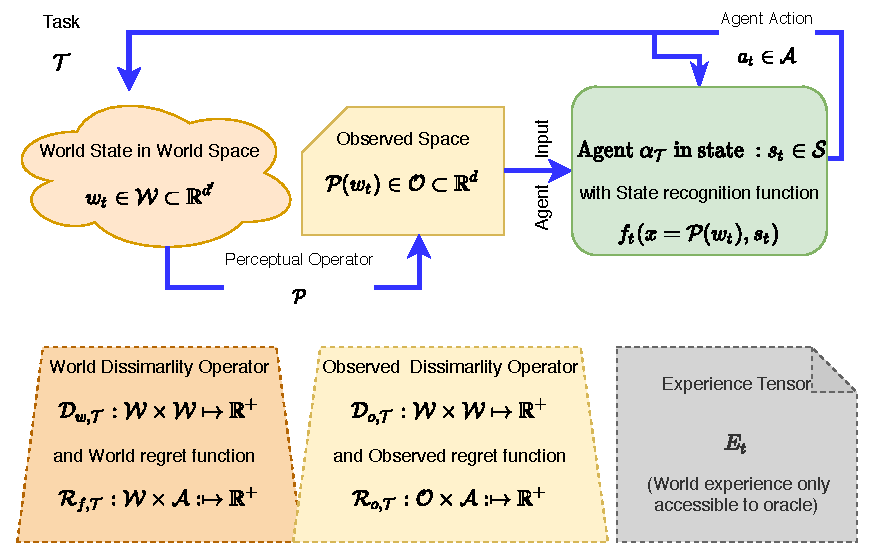
\includegraphics[width=\columnwidth]{Elements-of-novelty.pdf}
   \caption{Main elements of the implicit theories of novelty. The agent can only access world information indirectly through a perceptual operator ${\cal P}$. It can then update its internal state and act on the world state. Items with dashed outlines are outside of the task or agent but are critical to defining novelty.
In the framework a theory of novelty is obtained by specifying:
world $\cal W$ and the world dimensionality $d'$,
observation space ${\cal O}$ accessible to the agent and its dimensionality $d$, agent state space $\cal S$,
a perceptual operator ${\cal P}$ that processes world regions,
task-dependent world dissimilarity functions ${\cal D}_{w,{\cal T}}$ with associated threshold $\delta_w$,
task-dependent observation-space dissimilarity functions ${\cal D}_{o,{\cal T}}$ with threshold $\delta_o$,
agent $\alpha$ in state $s_t\in{\cal S}$ at time $t$, using
state recognition function $f_t(x,s)$ to determine the action $a_t \in{\cal A} $ to be taken, 
world regret function ${\cal R}_{w,{\cal T}}$, 
observation-space regret function ${\cal R}_{o,{\cal T}}$,
and agent-space regret function ${\cal R}_{a,{\cal T}}$. 
Every  set of these operators / functions / values defines a different theory of novelty for its associated task. 
}
\label{fig:elements}
\end{figure}


%We define the core elements  of the framework then present examples of it applied in domains then finally use the framework to define ten subtypes of novelty.


For simplicity of presentation, our world and observation space are $d'$ and $d$ dimensional spaces of real numbers. Let a world state be $w_t\in {\cal W}$, and let ${\cal W} \subset \real^{d'}, d'\ge d$, be the representation of the world state at time $t$ obtained from a subset of ${\cal W}$, the allowed world states. 
Note that $\cal W$ need not be the entire world. It can be only that region of space and time which is sampled during operation or that is relevant for the task. It could even be a finite set of items or relationships to be considered by the system. 


Let our observation at time $t$ be $x_t\in {\cal O}$ in observation-space ${\cal O} \subset \real^d $. 
%This generalizes the encoding of any computer system, including those for symbolic reasoning.  
Let ${\cal P}:\real^{d'} \mapsto \real^d$ be the perceptual operator at time $t$, which maps world spaces to observation spaces, \textit{i.e.}, ${x_t = {\cal P}}(w_t)$.  The agent never has direct access to the world and can only access it via the perceptual operator. 
%If one wants to consider a symbolic world state directly accessed by the agent, it would be formulated with the perceptual operator as the identity operator. However, in general, the perceptual operator is not information preserving as at least some world states are hidden. 
This operator is generally a combination of real-time sensing plus external processing on that sensed data. It can also include pre-processing on stored sensory data. But everything in this operator is to be considered external to the agent. Potential changes to system hardware can influence the outcomes of the perceptual operator and are represented as parameters of $\cal P$ stored within $w_t$. If the perceptual operator processes only a subregion of any world state, we let ${\cal W}_t$ be the subregion of the world that has been processed up to time $t$. Accordingly, any world states that differ only outside the processed subregions are indistinguishable.

 

Let agent $\alpha_{{\cal T}}$ solving task ${\cal T}$ at time $t$ have an internal state representation $s_t \in {\cal S}$, where ${\cal S}$ is the space of possible states.
An agent reacts to the environment, but a common architecture in the design of autonomous agents is for the agent to have an internal state $s_t$ that influences how the agent will act at time $t$. 
To capture this common agent architecture, we define a \emph{state recognition function} that maps an observation-space input, $x_t$, plus the current agent state, $s_t$, into its new internal state and action. 
% Formally, let $f_t(\cdot,\cdot ):\real^d\times{\cal S}\ \mapsto {\cal S}\times {\cal A}$ be a state recognition function at time $t$ mapping an observation-space input $x_t$ to its internal state space estimation $y$ of the world state $w_t$ yielding the  action $a_t \in {\cal A}$ to be taken to reach new state $s_t$, where $\cal A$ is the space of actions. 
Formally, let $f_t(x_t, s_t):\real^d\times{\cal S}\ \mapsto {\cal S}\times {\cal A}$ be a state recognition function at time $t$ mapping an observation-space input $x_t$ and its internal state $s_{t-1}$ to its new state $s_t$ and an action $a_t \in {\cal A}$ to be taken, where $\cal A$ is the space of actions. 


Based on the recognition function output, the agent takes an action. Then, the state transition function,
$T(w_t,a_t):{\cal W} \times {\cal A} \mapsto \cal W$, maps the current world state and agent's selected action at time $t$ to a new world state. 
This mapping can be stochastic, e.g., a Markov decision process.
Note that for many real problems the world may change outside of any assumptions, including oracle's assumptions, in which case we cannot assume $w_{t+1} = T(w_t,a_t)$.
For problems which traditionally do not have state transition function
or specify an action, such as machine learning or open set classification, agent's ``action" is the predicted outcome for a given sample, e.g., a class reported by the classifier. 
% Actions in learning systems may also update the parameters in the state or may change state recognition functions, which is why $f_t$ is a function of time~$t$.


Let $\cal N\subseteq \cal S$ be the possible empty set of internal states which are associated with the agent determining the world is novel. The world state $w_t$ is identified by the agent as novel if 
$s_t \in {\cal N}$.  When dealing with novelty, the agent may obtain unexpected observation states, which could map to potentially unexpected internal states (\textit{e.g.}, a ``crash'' state). 



To represent history, let $E_{t} = \{(w_1) \ldots (w_t)\}$ be our experience tensor of states. 
It is important to note that the experience tensor is not about what the agent ``remembers''.
 It is external to the agent and is about what world states the agent has experienced up to and including time $t$. 
The experience tensor is integral to defining novelty, which depends on dissimilarity between the potentially novel world and the experience of some non-novel worlds.



%Any agent memory is captured in state vector $s_t$ and potentially in an updated recognition function $f$. 
%The agent's model need not even try to estimate $\cal W$ if such modeling is not needed for its task; an agent with no inputs can still have state and state estimation. 

\section{Dissimilarity and Regret Measures}
For a given task ${\cal T}$, data generally do not need to match exactly to be considered ``the same'' with respect to the task's objectives.  Note that while we call it ``a task,'' it could include a set of objectives (\textit{e.g.}, a multi-task problem). In any task, multiple dimensions can impact the task performance and determine when a state is effectively the same or how different a state is from prior experience.  We formulate this in terms of a measure of dissimilarity, which depends on the task. It is important to note that one should be careful in {\em a priori} definitions of what matters to a task, as novel world states may have an unpredictable impact on it. 

Essential to our framework is a set of task-dependent dissimilarity functions ${\cal D}_{w,{\cal T}}:{\cal W}\times {\cal W} \mapsto \real^+$ and ${\cal D}_{o,{\cal T}}:{\cal W}\times {\cal W} \mapsto \real^+$, which measure dissimilarity between states in the world space and the observation space respectively.  The perceptual dissimilarity may access the world but must map to observed space with the perceptual operator before mapping to $\real^+$. 
Both dissimilarities can use experience tensor $E_t$ as an optional parameter.
Dissimilarity measures produce non-negative values that are a generalization of distance metrics. It is possible to have zero dissimilarity for states that are identical in terms of the task and hidden variables, even if they are distinct states in the world or observation space. Novelty definitions will generally include a similarity threshold of $\delta_w$ and $\delta_o$, beyond which a state is treated as novel, which depends on the task and user requirements.
Dissimilarity may be an actual distance metric, a statistical measure, an information-theoretic measure, or such measures combined with ontological or hierarchical information.  If the world modeling is probabilistic, then the dissimilarity function may, but need not, be based on probabilistic computations.   
We use dissimilarity rather than distance since it is well known that human perception / recognition is non-metric~\cite{tversky1977features,scheirer2014good}. %Note the dissimilarity functions can be parameterized to include the experience tensor, thereby allowing them to use statistical measures, estimated dynamics, or other measures over the experiences in determining dissimilarity. 
% Dissimilarity measures produce non-negative values that are a generalization of distance metrics. It is possible to have zero dissimilarity for items that are identical in terms of the task, even if they are distinct items in the world / observation space.  Novelty definitions will generally include a similarity threshold of $\delta$ on the maximum allowed dissimilarity for items treated the same by the task, which depends on the task / user requirements for matching.
% Dissimilarity may be an actual distance metric, a statistical measure, an information-theoretic measure, or such measures combined with ontological or hierarchical information.  If the world modeling is probabilistic, then the dissimilarity function may, but need not, be based on probabilistic computations.   
% We use dissimilarity rather than distance since it is well known that human perception / recognition is non-metric~\cite{tversky1977features,scheirer2014good}. 






Not all novel states are of interest or present a risk to the agent.
While we cannot know the risk of an unknown state until it becomes known, we can, after the fact, assign a regret score associated with new world / observed / agent state after the action $a_t(w_t,s_t)$. 
We let ${\cal R}_{f,{\cal T}}:({\cal O} \times {\cal A} )\mapsto\real$, ${\cal R}_{o,{\cal T}}:({\cal O}\times {\cal A} )\mapsto\real$ and ${\cal R}_{w,{\cal T}}:({\cal W} \times {\cal A} )\mapsto\real$ be the regret operators for task ${\cal T}$ in agent, observation, and world space respectively. Agent and observation regrets are functions of an observed state, whereas world regret of a world state. A suboptimal agent may have an agent regret higher than an observation regret, which should be defined with respect to an oracle or the best agent on observed data.   

We separate these three because it allows one to reason about regret in terms of specific models. Only an oracle that has access to ground-truth data has the ability to actually compute regret in world space. However, an agent can approximate regret in observation space, especially given the ground-truth answers. It is important to note that agent-computed regret can only be an approximation, even given the ground-truth action / outcome, because the optimal decision with limited data can still lead to bad outcomes. Hence, an agent might estimate regret even if there should be none. 




\section{Example: CartPole Domain}



As an example of using the constructs defined above, consider  the 
CartPole in the OpenAI Gym.\footnote{\url{https://github.com/openai/gym/blob/master/gym/envs/classic_control/cartpole.py}} 
In this domain, a cart has a pole connected to it, and the task ${\cal T}$ is to push the cart left or right so as to prevent the attached pole from falling. 
The world state $w$ in the CartPole domain comprises the following real values (with default / initial values in parentheses): 
gravity $G~(9.8)$, 
mass of cart $M_c~(1.0)$, 
mass of pole per unit length $M_p~(0.1)$,
length of pole $L~(1.0)$,
force of push $F_p~(10.0)$,
horizontal force acting on the cart $F_h~(0)$,
min / max cart position $z^{\text{min}} (-2.4), z^{\text{max}} (+2.4)$,
min / max pole angle $\phi^{\text{min}}$ ($-12^{\circ}$), $\phi^{\text{max}}$ ($+12^{\circ} $),
time between state updates $\tau$ ($0.02$ seconds), 
start time $t$ (0). The
initial cart position $z_0$, 
 cart velocity $\dot{x}_0$, 
 pole angle $\phi_0$, 
and  pole angular velocity $\dot{\phi}_0$ are all i.i.d. random samples from  $[-0.05...0.05]$.
The perceptual operator ${\cal P}$ in this domain is a projection of the world state that returns only the cart position $z$, cart velocity $\dot{z}$, pole angle $\phi$, and pole angular velocity $\dot{\phi}$ as the 4D observed state vector  $x=(z, \dot{z}, \phi, \dot{\phi})$. 

Based on these world state features, the task is more precisely defined as: given $x$, select an action from the space of ${\cal A}=\{\text{Left},\text{Right}\}$  to maintain the cart position within the min / max cart position and maintain the pole angle within the min / max pole angle. Note that the last four features (cart position, cart velocity, pole angle, pole angular velocity) are determined via a  deterministic physics model based on the full world state combined with agent actions.


\subsection{Dissimilarity and Regret in CartPole}

State transitions in the CartPole domain are determined by the equations of motion and can be simulated in discrete time with numerical integration.
In this example we  assume transitions between observed states are Markovian, which simplifies presentation;   other theories for this domain could consider dissimilarity and regret in more general settings. 

% {\cal D}_{w,{\cal T}}
The dissimilarity measure for CartPole might take a simple form (\textit{e.g.}, the Euclidean distance in the world or observed space).
% why conditioning is important?
% One outcome of the formalization effort was the observation that an evaluation using Euclidean distance between initial world states to define novelty  does not capture ``difficulty.'' 
However, Euclidean distance between world states is affected by factors  other than novelties,
% This is because the measure is dependent on the choice of units and is insensitive to the  variation in the impact of different variables on the state evolution or task outcome.
including  the choice of units. It is also insensitive to the  variation in the impact of different variables on the state evolution or task outcome.  
Proper conditioning would reduce dependency on units and account for states that correspond to different samples from the same world (\textit{e.g.}, the same CartPole world with a different initial position of the pole is not considered novel).

% conditioning
To avoid these issues, we compare two worlds, $w$ and $\check{w}$, the states that proceed from a common observed state and action.
We consider an action of an optimal agent,~$a^*$, in the first world, $w$, and choose as the common observed states the states that the agent encounters,~$\check{x}_t$, in the second world, $\check{w}$.
Then, we average over all these states, including the initial observed state:
% We choose this configuration, because it corresponds to an agent having an expectation about the next state, $T()$, given the previous state and action, $x_{t-1}$, $a_{t-1}$.
%This dissimilarity measure can be seen as a state prediction error under quadratic loss, $\ell_{\cal S} (x_{t-1}, a_{t-1}, \check{x}_t)=(\check{x}_t-x_t)^2$.
% optimal agents
% A better dissimilarity measure selects an agent that is optimal for the world in the function's first argument, then simulates and averages that optimal agent's behavior over starting states in the world of the second argument:
\begin{align*}
%   {{\cal D}}_{w,{\cal T};E_{t-1}}(\check{w}_t, w_t) =
%   \E_{t,w_0} (\check{A}(\check{w}_{t-1})-w_t)^2. \\
%   {{\cal D}}_{o,{\cal T};E_{t-1}}(\check{w}_t, w_t) =
%   {{\cal D}}_{o,{\cal T}}(W, W') =
%   \E_{t,w_0} (  {\cal P}(T(w_t',a^*_{t})) - {\cal P'}(T'(w_t',a^*_{t}))^2
 {{\cal D}}_{o,{\cal T}}(w, \check{w}) =
\E_{\check{x}_0,t} 
(
 &{\cal P}(T(M(w,\check{x}_t),a^*_{t}) - \\
 &{\cal P}(T(M(\check{w},\check{x}_t),a^*_{t}) 
 )^2,
\end{align*}
where $M(w,x):{\cal W} \mapsto {\cal W}$ is a function that returns a  modified $w$ whose observed components are replaced with the values from $x$, such that ${\cal P}(M(w,x))=x$, while all other components remain unchanged. 
Overall, the dissimilarity measures the average distance between observed states in two different worlds that proceed from a common observed state and action,~$\check{x}_t$ and $a^*_t$.
The agent is optimal in the first world, while the trajectory is from the second world, so this dissimilarity measure can be seen as an expected state prediction error of the optimal agent trained in the first world and tested in the second world.
% We let   ${{\cal D}}_{o,{\cal T};E_{t-1}}(\check{x}_t, x_t)=   {{\cal D}}_{w,{\cal T};E_{t-1}}(\check{w}_t, w_t)$, where the oracle can expand $\check{x}_t$ and $x_t$ to the associated world states and run a simulation to get averages for the expected value. 
% 
The world dissimilarity is defined analogously, except it does not use the perceptual operator.
% experience tensors
Note that these dissimilarity measures depend on multiple experience tensors of the respective optimal agents, i.e., the average is over their trajectories.

This is an asymmetric dissimilarity measure as the selected agent is optimal for the first world and need not be optimal for the second, and then marginalizes over the initial conditions and time in the second world.
Due to the conditioning, any pair of states from the same world will have zero dissimilarity. Furthermore, since these depend on the choice of ``optimal action'' $a^*_{t}$ from the first world,  it implicitly normalizes for how different dimensions (variables) impact the evolution of the world state. 
% Note that the states encountered in the time period between $t-1$ and $t$ depend on the agent and $\cal T$. 
One can consider actions of an optimal reference agent under given conditions (\textit{e.g.}, a non-adaptive agent that performs optimally w.r.t. the main task $\cal T$ in a non-novel CartPole world.
If it is infeasible to obtain an optimal agent in practice, then one may use an arbitrary reference agent and its expectation, with the caveat the dissimilarity measure will depend on the oracle's reference agent. 


% probabilistic transition function - towards a regret
% If the world is intrinsically probabilistic and unpredictable, e.g., the state transitions are governed by a Markov decision process, then this dissimilarity can be non-zero, even though $x$ and $x'$ are the same worlds without any novelty. To avoid this issue, 
% the more general dissimilarity measure separates the predictable and noisy parts of the state transitions, and integrates out the noise, 
% \begin{equation}
%     % {\cal D}_{w,{\cal T};E_{t-1}} (w_t, \check{w}'_t) = \E_{\check{w}_t|w_{t-1}} (w_t-\check{w}_t)^2 - (\check{w}'_t-\check{w}_t)^2,
%     {\cal D}_{o,{\cal T};E_{t-1}} (x_t, \check{x}'_t) = \E_{x'_t|x_{t-1}} (x_t-x'_t)^2 - (\check{x}'_t-x'_t)^2,
%     \label{eq:Dw_nondet}
% \end{equation}
% where $\check{w}_t'$ is an asymptotic predictor of $\check{w}_t$. Note that the second component of the sum is zero and we retain Eq.~\ref{eq:Dw_det}, if the state transition function is deterministic, as in Cart Pole.

% a link to regret
% Interestingly, each of the last two equations is a difference of two loss functions, so they can be written as
% \begin{align}
%     % {\cal D}_{w,{\cal T};E_{t-1}} (\check{w}_t, \check{w}'_t) &= 
%     % \ell_{\cal S} (\check{w}_t) - \ell_{\cal S} (\check{w}'_t),\\
%     {\cal D}_{o,{\cal T};E_{t-1}} (\check{x}_t, \check{x}'_t) &= 
%     \ell_{\cal S} (\check{x}_t) - \ell_{\cal S} (\check{x}'_t).
%     \label{eq:DwDx}
% \end{align}
% where $\ell_{\cal S} (\check{w}_t) = \E_{\check{w}_t|w_{t-1}} (\check{w}_t-\check{w}_t)^2$ is a quadratic loss. 

% state prediction
%In general, the task $\cal T$ is different from the task of state prediction. 
% While an agent need not have an  explicit next state prediction function, state prediction could  help in achieving a better performance at $\cal T$. In addition, it could be used for novelty detection which might be a required secondary task. The two tasks overlap to some extent, \textit{e.g.}, in Cart Pole the observed state includes four variables, but predominantly one of them, pole angle, needs to be predicted and constrained to keep the pole straight.
% The loss $\ell_{\cal S}$ measures the error, or regret, for a selected action $a_t \in {\cal A}$ in a given state.

% regret
Regret for the agent's action at state $x_t$ w.r.t. $\cal T$ is
\begin{align}
    {\cal R}_{o,{\cal T}} ( x_t, a_t) = 
    % {\cal R}_{w,{\cal T}} ( w_t, a_t) = 
    \ell_{\cal T} (x_t, a_t) - \ell_{\cal T} (x_t, a^*_t),
     \nonumber
    \label{eq:Rx}
\end{align}
where $\ell_{\cal T} (x_t, a_t)$ is the loss incurred in the state $x_t$ by an agent that performs action $a_t$, while $\ell_{\cal T} (x_t, a^*_t)$ is the loss of an agent that performs the optimal action $a^*_t$, given the same observation.
In CartPole, the loss at the given time step is $1$ if the pole angle or cart's position in the next time steps is beyond the threshold, $|\phi|>\phi^{\text{max}}$ or $|z|>z^\text{max}$, otherwise the loss is $0$.
In this CartPole domain, the world regret is the same as observation regret, ${\cal R}_{w,{\cal T}} ( w_t, a_t) = {\cal R}_{o,{\cal T}} ( {\cal P}(w_t), a_t)$, because there are no hidden dynamic elements interacting with pole or cart, such as an invisible pendulum that hangs above the pole and sometimes hits it. Once such elements are introduced, the two regrets may differ.
% Hence, the regret of an optimal agent trained in the novel world is zero.



\begin{figure}
    \centering
    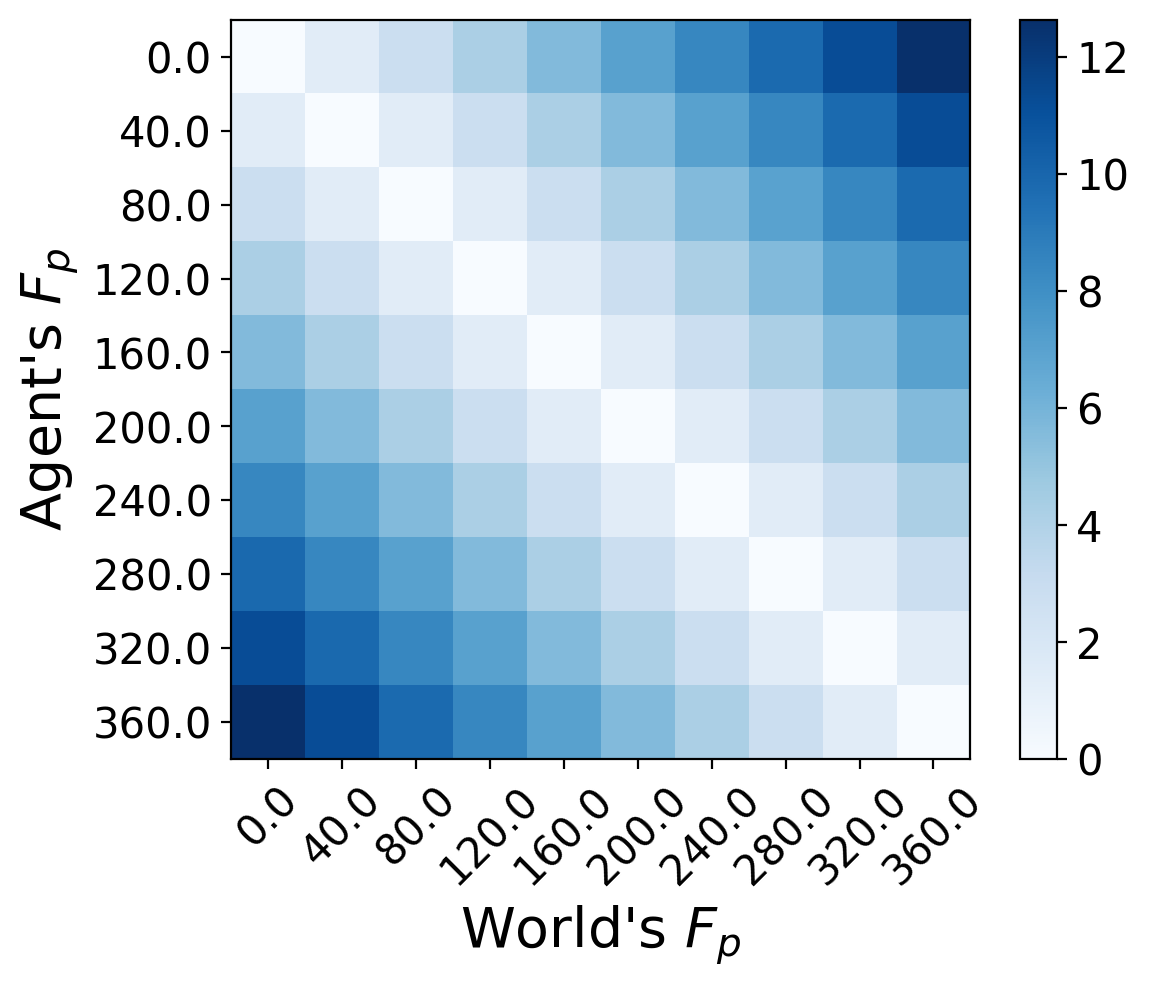
\includegraphics[width=.49\columnwidth]{images/dist_action_force_mag.png}
    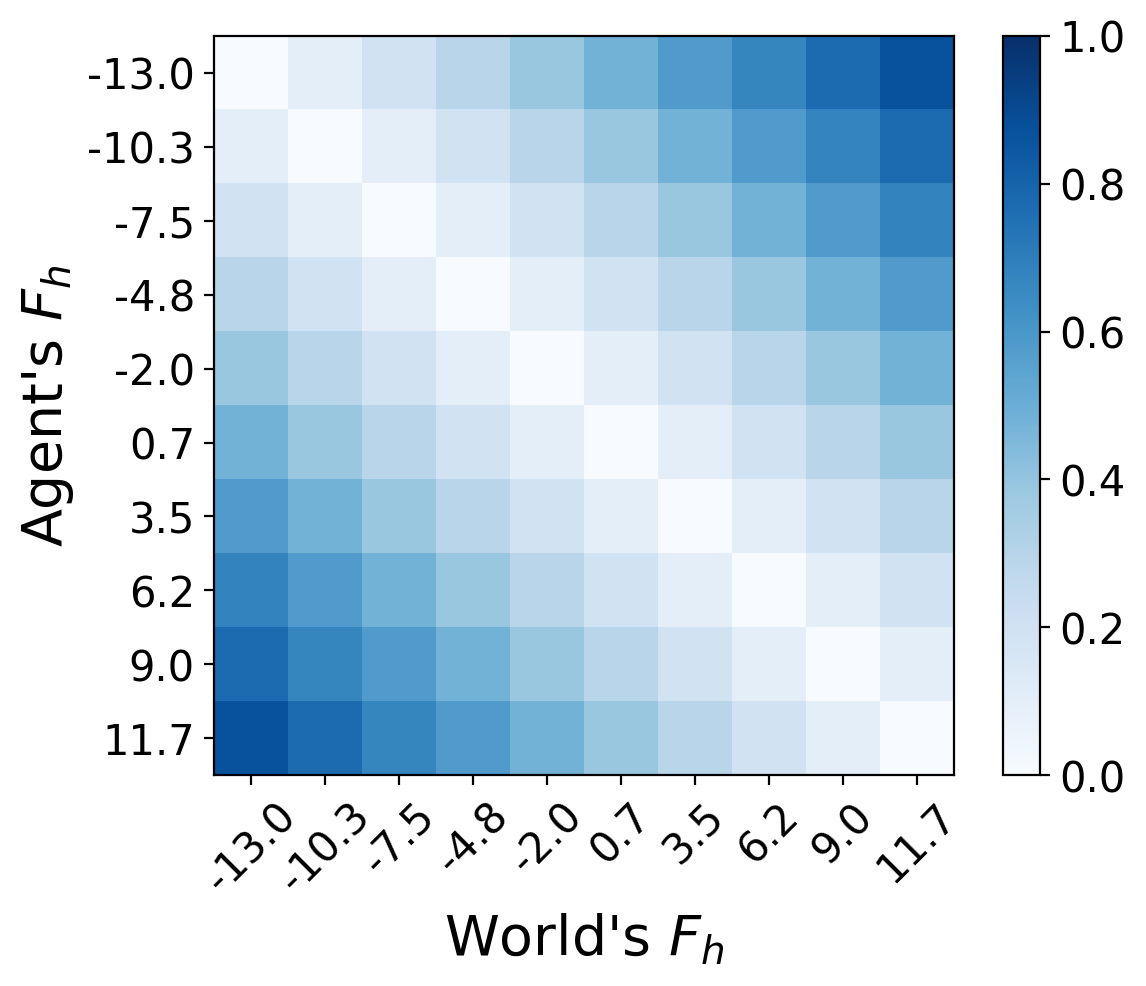
\includegraphics[width=.49\columnwidth]{images/dist_env_force.png}
    \caption{Observation dissimilarity, $ {{\cal D}}_{o,{\cal T}}(w, \check{w})$, between a world expected by an optimal non-adaptive agent and the observed world. The agents are optimal in a world having incorrect value of the magnitude of pushing force, $F_p$ (left panel), or a horizontal force acting on the cart, $F_h$ (right panel). The expectation is computed over 20 samples of the initial world state $w_0$.}
    \label{fig:diss}
\end{figure}

\begin{figure}
    \centering
    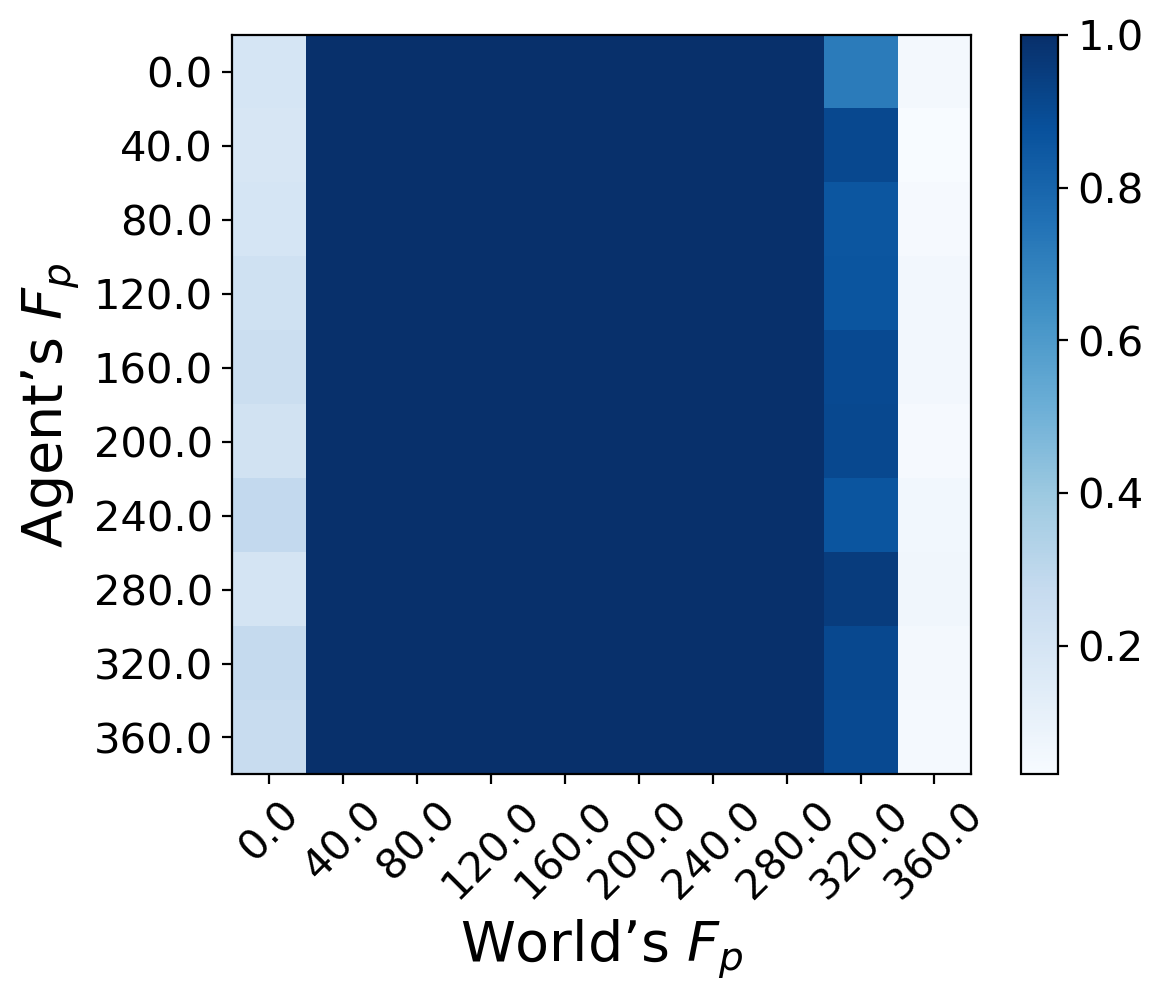
\includegraphics[width=.49\columnwidth]{images/regret_action_force_mag.png}
    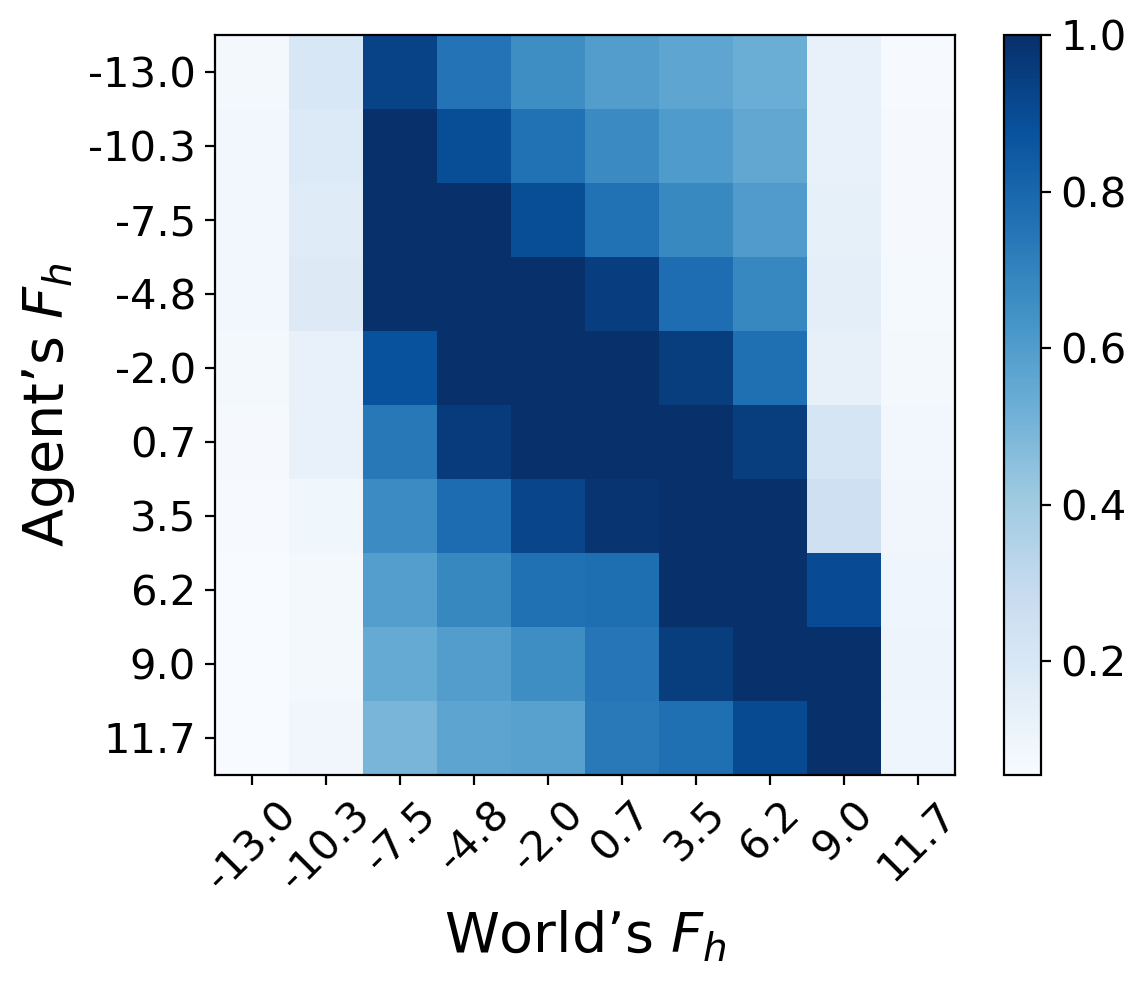
\includegraphics[width=.49\columnwidth]{images/regret_env_force.png}
    \caption{Average reward, 1-$\E_{x_0,t} \ell_{{\cal T}} ( x_t, a^*_t) $, of non-adaptive agents that are trained to act optimally in a certain world but are tested in another world.}
    \label{fig:regret}
\end{figure}

\subsection{Agent State and Optimal Non-Adaptive Agents}

% In CartPole, the state transition function has latent parameters such as gravity, pole length, push force magnitude, masses, friction, strength of a horizontal force (wind), etc. The changes to these latent variables can be interpreted as explicit novelties. 

In simple environments, like CartPole, it is possible to obtain optimal or near-optimal non-adaptive agents. A particularly simple version of CartPole is the one where the agent’s action space is binary, \textit{i.e.}, the agent can choose to push the cart left or right, and its reward is the time that the pole is up. In such a CartPole environment, an agent can find optimal actions by performing what-if simulations of the world and searching for actions that result in the best performance, \textit{i.e.}, the agent can simulate what would happen if it pushed the cart left or right and then choose the next action that results in better performance.  In this paper, for simplicity, we present the results for a near-optimal single-look-ahead agent. 
% This agent assumes the full knowledge of the non-novel world and it is able to simulate the non-novel world with high fidelity. 
The action is chosen based on the distance, $||\beta^\intercal (x_t-x^\text{s})||$, between the expected state resulting from the action, $x_t$, and the desired state, $x^\text{s}=(0,0,0,0)$, where the weight vector $\beta=(0,0,1,0.005)$ weighs discrepancy in $\phi$ the most and ignores the discrepancies in $z$ and $\dot{z}$.
The state of this agent is described by the parameters used to simulate system dynamics and the weight vector, $s=(G, M_c, M_p, L, F_p, F_h, \tau, \beta)$. In non-adaptive agents, these parameters are fixed to the values that correspond to the non-novel world. 
% Adaptive agents can learn the values of these parameters on-the-fly as they interact with the environment.

\subsection{Measurements and Observations}

% dissimilarity
As expected, the observed dissimilarity captures the novelties in the magnitude of pushing force and in a horizontal force acting on the cart (Figure~\ref{fig:diss}). The larger the distance between the value of a given parameter in the world and its value assumed by the agent, the larger the dissimilarity in state prediction.

% ignorable novelties
Surprisingly, in CartPole, reasonable changes to many of the aforementioned latent parameters, like the gravity or the magnitude of pushing force, do not impact an optimal non-adaptive agent’s performance (left Figure~\ref{fig:regret}). 
% vertical bars and domain limits
The columns on the verge of the heat map correspond to the achievable limits in performance, \textit{i.e.}, the leftmost column corresponds to such a small force magnitude that the push is insufficient to counter the gravity, whereas the rightmost column corresponds to such a large force magnitude that the push instantly rotates the pole beyond the allowed region.
We conclude that the optimal agent performs just as well in the novel world where gravity or pole length have new values, despite making simulations that assume incorrect values of gravity or pole length, \textit{i.e.}, the values from the non-novel world. 
Note that this agent is non-adaptive, so it does not change its internal model to adapt to the novel world, \textit{i.e.}, internally it uses the model of the non-novel world to take actions.
Again, the columns at the verge of the heat map mark inherent performance limits, \textit{i.e.}, if the magnitude of the horizontal force is larger than the pushing force, $|F_h|>F_p=10$, then the pushes are insufficient to counteract the horizontal force and the pole is destined to fall, despite taking optimal actions.

% novelties impacting agent performance
Less surprisingly, some of the latent parameters impact the agent’s performance in an intuitive way (\textit{e.g.}, a horizontal force applied to the cart) (right Figure~\ref{fig:regret}). This happens because the horizontal force directly impacts the action that the agent should choose: if the horizontal force pushes the cart right, then the agent should probably push it left, and vice versa. The larger the difference between the horizontal force in the environment and assumed by the agent, the higher the drop in the agent's performance.

% regret dissimilarity
To distinguish between novelties that affect or do not affect the task performance, we use the regret of an optimal agent trained in the non-novel world and tested in the novel world, \textit{i.e.}, ${\cal R}_{o,{\cal T}} ( x_t, a^*_t) $. Novelties with ${\cal R}_{o,{\cal T}} ( x_t, a^*_t) = 0$ do not affect task performance and can be ignored by agents that are near-optimal without a performance drop.
% dissimilarities
By contrast, ${\cal R}_{o,{\cal T}} ( x_t, a^*_t) > 0$ tells us that the novelty impacts the performance of an optimal non-adaptive agent and that the agent can update its state to improve its performance, \textit{i.e.}, learn the novelty.
% adaptive agent
Naturally, one can develop an adaptive version of this agent by learning an estimate of world state parameters
% , $s\approx w_0$, 
from observations and using them to perform more accurate simulations and taking better actions. %Such an agent can learn on-the-fly and adapt to the  environment, maintaining low regret. 
%A crucial research problem is to develop efficient adaptive agents.

% momentous and asymptotic regret
% Their world and perceptual regret can be computed both in an asymptotic and momentous manner, i.e., we can measure the asymptotic regret of this agent or we can measure how its regret was evolving with the number of samples after the introduction of novelty. 


% task 1: keep pole straight (prediction of pole angle, i.e., a part of observed state)
% novelty not impacting performance: force magnitude
% impacting performance: force offset (a wind)

% task 2: novelty detection as world comprehension (prediction of full observed state)
% all novelties impact performance
% multiple world dissimilarities for the same task
% identifiability issue: force magnitude vs cart weight (if friction not present)
% the importance of observations and actions for identifiability

% examples:
% "An imperceptible novelty is when there is a large change in the world model that doesn’t result in a change to the perceptual features, e.g., tweak all the world parameters a little bit, or in ways that oppose each other (more gravity, less friction)". Increase in gravity isn't equivalent to decrease in friction, because gravity also impacts the pole. Perhaps a more fitting example: an increase in cart mass is equivalent to a respective decrease in force magnitude, if there is not friction. This case is "imperceptible" if there is something in the world that doesn't affect observations, but is affected by mass or force magnitude. If such thing doesn't exist, then I don't think this case is novelty, since one could argue than no physical law has changed, just the units of cart mass and force magnitude have changed.

\if{0}
\subsection{Agent State}
The set of internal states ${\cal A}$ depends on the implementation of the agent. For our example, consider a simple DQN-based agent that runs for $N$ iterations to train a DNN to output the Q value of each action, 
and from iteration $N+1$ and onward chooses actions greedily according to learned network. 
Let DNN$_i$ be the trained network as iteration $i$. 
The internal state of the agent in iteration $i\leq N$ comprises all the observation-space states collected ($E_{o,t}$) and the so far and the current DNN (DNN$_i$). 
After the $N$th iteration, the agent's internal state is only the learned DNN, as the agent chooses its actions according to the DNN and the given observation-space state.   Formally, 
\begin{equation}
f_t(x : E_t) = 
\begin{cases}
(E_t, DNN_t) & \text{if $t\leq N$} \\
DNN_{100} & \text{if $t> N$} 
  \end{cases}
\end{equation}
% The state recognition function $f_{y,t}(x = P(w) : E_t)$ maps directly to the sensors of interest, but there are likely several states $y$ consistent with a perceived feature vector $x$.
% The family of actions $a_t(x)$ taken by agent $a_f$ are ``left'' or ``right,'' which correspond to an instantaneous push of the cart in the corresponding direction with force $F_p$.
The actions the agent can take at any time $t$ are ``left'' or ``right,'' which correspond to an instantaneous push of the cart in the corresponding direction with force $F_p$.
The world regret function $R_{w,T}$ is based on whether $x$ or $\phi$ exceed their bounds in $w$. This can be a Boolean (success / failure) or a score based on the amount of time that $x$ and $\phi$ remain within bounds. The observation space regret function $R_{f,T}$ has the same value as $R_{w,T}$, but is not necessarily determined by $f$. %cannot necessarily be determined by $f$.
\fi




% Please add the following required packages to your document preamble:
% \usepackage{multirow}
{
\renewcommand{\arraystretch}{1.15}
\begin{table*}[] \centering 
\begin{tabular}{|c|c|c|c|c|c|c|}
\multicolumn{1}{|c|}{\multirow{4}{*}{\rotatebox[origin=c]{90}{ \parbox{.2in}{World\\ Novelty}}}}&\multicolumn{1}{l|}{\multirow{2}{*}{\rotatebox[origin=c]{90}{\hspace{-6ex}\parbox{.2in} {Observation\\ Novelty}}}}& \multirow{2}{*}{\rotatebox[origin=c]{90}{\hspace{-6ex}\parbox{.2in}{Agent\\ Novelty}}} & 
\multicolumn{2}{c}{ World Regret ${\cal R}_{w,{\cal T}} > \epsilon_w$} & \multicolumn{2}{|c|}{{{No World Regret ${\cal R}_{w,{\cal T}} \le \epsilon_w$}}}          \\ \cline{4-7}
&&&\parbox{1.2in}{\vspace{2pt} \centering Perceptual Regret\\${\cal R}_{o,{\cal T}} > \epsilon_o$}
&\parbox{1.2in}{\vspace{2pt} \centering No Perceptual Regret\\${\cal R}_{o,{\cal T}} \le \epsilon_o$}
&\parbox{1.2in}{\vspace{2pt} \centering Perceptual Regret\\${\cal R}_{o,{\cal T}} > \epsilon_o$}      
&\parbox{1.2in}{\vspace{2pt} \centering No Perceptual Regret\\${\cal R}_{o,{\cal T}} \le \epsilon_o$}\\ \hline
\multicolumn{1}{|c|}{\multirow{4}{*}{\rotatebox[origin=c]{90}{{Yes }}}}     & \multicolumn{1}{l|}{\multirow{2}{*}{\rotatebox[origin=c]{90}{Yes}}}   & \multicolumn{1}{l|}{  Yes}  & \multicolumn{1}{l|}{Unanimous w/ Regret}                & \multicolumn{1}{l|}{Unanimous  Nuisance}      & \multicolumn{1}{l|}{Unanimous  Nuisance}      & \multicolumn{1}{l|}{Unanimous Managed}             \\ \cline{3-7} 
\multicolumn{1}{|c|}{}                                   & \multicolumn{1}{l|}{}                                      & \multicolumn{1}{l|}{  No} & \multicolumn{1}{l|}{Ignored}                  & \multicolumn{1}{l|}{Ignored Nuisance}         & \multicolumn{1}{l|}{Ignored Nuisance}         & \multicolumn{1}{l|}{Ignored Managed}               \\ \cline{2-7} 
\multicolumn{1}{|c|}{}                                   &
\multicolumn{1}{l|}{\multirow{2}{*}{\rotatebox[origin=c]{90}{No}}} 
  & \multicolumn{1}{l|}{  Yes }  & \multicolumn{1}{l|}{Imperceptible}             &   \multicolumn{1}{l|}{Imperceptible Nuis.}             & \multicolumn{1}{l|}{Imperceptible Nuis.}             & \multicolumn{1}{l|}{Managed Imperceptible}          \\ \cline{3-7}
\multicolumn{1}{|c|}{}                                   & \multicolumn{1}{l|}{}                                      & \multicolumn{1}{l|}{  No } & \multicolumn{1}{l|}{Imperceptible Ignored }     & \multicolumn{1}{l|}{Imper. Ignored Nuis.}     & \multicolumn{1}{l|}{Imper. Ignored Nuis.}     & \multicolumn{1}{l|}{Managed Imperceptible} \\ \hline
\multicolumn{1}{|c|}{\multirow{4}{*}{\rotatebox[origin=c]{90}{{No}}}} &
\multicolumn{1}{l|}{\multirow{2}{*}{\rotatebox[origin=c]{90} {Yes}}} 
  & \multicolumn{1}{l|}{  Yes}  & \multicolumn{1}{l|}{Faux}                     & \multicolumn{1}{l|}{Faux Nuis.}                     & \multicolumn{1}{l|}{Faux Nuis.}                     & \multicolumn{1}{l|}{Managed Faux}                  \\ \cline{3-7} 
\multicolumn{1}{|l|}{}                                   & \multicolumn{1}{l|}{}                                      & \multicolumn{1}{l|}{  No} & \multicolumn{1}{l|}{Faux  Ignored}            & \multicolumn{1}{l|}{Faux  Ignored Nuis.}            & \multicolumn{1}{l|}{Faux  Ignored  Nuis.}            & \multicolumn{1}{l|}{Managed Faux}          \\ \cline{2-7} 
\multicolumn{1}{|l|}{}                                   &
\multicolumn{1}{l|}{\multirow{2}{*}{\rotatebox[origin=c]{90}{No   }}}
  & \multicolumn{1}{l|}{Yes}  & \multicolumn{1}{l|}{Faux}                     & \multicolumn{1}{l|}{Faux  Nuis.}                     & \multicolumn{1}{l|}{Faux  Nuis.}                     & \multicolumn{1}{l|}{Managed Faux}                  \\ \cline{3-7} 
\multicolumn{1}{|l|}{}                                   & \multicolumn{1}{l|}{}                                      & \multicolumn{1}{l|}{No} & \multicolumn{1}{l|}{\parbox{1.in}{ \vspace{2pt} No novelty } } & \multicolumn{1}{l|}{No novelty  Nuis. } & \multicolumn{1}{l|}{{\parbox{1.in}{ \vspace{2pt} No novelty  Nuis. } } } & \multicolumn{1}{l|}{No Novelty}                    \\ \hline
\end{tabular}
\caption{Subtypes of novelty defined by interaction of primary novelty types and regret. 
Some combinations of states get multiple labels (\textit{e.g.}, Unanimous  Nuisance is both Unanimous (all types of novelty present) and Nuisance (inconsistent regret values)).
}
\label{tab:types}
\end{table*}
\renewcommand{\arraystretch}{1}
}



\comment{
\begin{figure}
 \centering
   \includegraphics[width=.9\columnwidth]{novelty_venn_diagram.pdf}
   \caption{Diagram highlighting the formally defined types of novelty and the relation to the primary world-level novelty, perceptual-level novelty, and agent-level novelty. 
   The black dashed line indicates the area of faux novelty.
  \label{fig:types}
 }
\end{figure}
}


\section{Types of Novelty} 
For the definitions, we introduce the primary types of novelty, with the subtypes defined by combining primary types and regret (see Table~\ref{tab:types} and \cite{Boult-eta-al-novelty20}).
%Fig.~\ref{fig:types}.
Using our definitions of world, observation space, internal states, and the corresponding dissimilarity functions, we can formally define the following primary types of novelty.  
%

%{\bf World-level novelty}, \textit{i.e.}, actual novelty, for an agent $\alpha$ at time $t$, is defined as any world state $\check{w}\in{\cal W}$ such that $\delta_w < \min_{w \in E_t} {\cal D}_{w,{\cal T}} (w,\check{w}; E_{t})$. That is any world state $\check{w}$ that is dissimilar from every state in the experience tensor. Note only an oracle with access to $E_t$ and ${\cal D}_{w,{\cal T}},$ can determine that something is truly novel. We note that if the world representation is viewed as including distributional information, \textit{e.g.}, probabilities of various items occurring, then a change in distributional parameters can be a world-level novelty even if no new ``objects'' occur in the world. Thus world-level novelty can produce problems of domain adaption, not just domain transfer.

{\bf World novelty.} A world state $\check{w}\in{\cal W}$ is considered a world novelty for agent $\alpha$ at time $t$ if $\min_{w \in E_{t-1}} {\cal D}_{w,{\cal T}} (w,\check{w}; E_{t-1}) > \delta_w$. That is, any world state $\check{w}$ sufficiently dissimilar from every world state in the experience tensor is a world-level novelty. Only an oracle with access to $E_{t-1}$ and ${\cal D}_{w,{\cal T}}$ can determine that a world state is truly novel. If the world representation is viewed as including distributional information (\textit{e.g.}, probabilities of various items occurring) then a change in distributional parameters can be a world-level novelty even if no new ``objects'' occur in the world. Thus world-level novelty can produce problems of domain adaption, not just domain transfer.

% {\bf Perceptual-level novelty}, \textit{i.e.}, observation-level novelty, for an agent $\alpha$ at time $t$, is defined as any observation vector $x={\cal P}(\check{w}\in{\cal W})$ such that $\delta_o < \min_{w_i \in E_t} {\cal D}_{o,{\cal T}} (x,{\cal P}(w_i);E_t)$.
% {\bf Observation novelty.} An observation space state $x={\cal P}(\check{w}\in{\cal W})$ is considered an observation novelty for an agent $\alpha$ at time $t$ iff $\min_{w_i \in E_t} {\cal D}_{o,{\cal T}} (x,{\cal P}(w_i);E_t) > \delta_o$.
{\bf Observation novelty.} A world state $\check{w}\in{\cal W}$ is considered an observation novelty for an agent $\alpha$ at time $t$ iff $\min_{w \in E_{t-1}} {\cal D}_{o,{\cal T}} (w,\check{w};E_{t-1}) > \delta_o$.
That is, an observation novelty is the observation-space state obtained for any world state $\check{w}$ that, when projected through a perceptual operator, is sufficiently dissimilar from every observation-space state in the agent's experience tensor.
Note that in this definition, the observed world state, $\check{w}$, is subject to the current perceptual operator ${\cal P}$ at time $t$ and is compared to the observation-space states in the experience tensor, which may have used the perceptual operator with potentially different parameter values (stored in world states).
It is not surprising that the same world state may be novel at one point in time but not novel at another. However, it may be surprising that if the perceptual operator changes over time, then something can be perceptually novel at time $t$ even if it was not perceptually novel at time $t-1$. For example, consider a transmission glitch creating errors in a static scene that has been viewed previously.
It is important to note that observation novelty is defined considering all experience, which permits observation novelty that includes distributional shifts or reasoning about consecutive states to detect novelty in dynamics.  
If the agent had access to the true dissimilarity ${\cal D}_{o,{\cal T}}$, it could use that to define its state recognition function $f$.  However, in practice, an agent will not have access to ${\cal D}_{o,{\cal T}}$, since it is trying to learn such a function from the data or was programmed with static rules to approximate it. Furthermore, agents rarely store all inputs. 


{\bf Agent novelty.} An observation-space state $x={\cal P}(\check{w}\in{\cal W})$ is considered an agent novelty for an agent $\alpha$ at time $t$ {\em iff} $f_t(x) = {\cal N}$. That is, $x$ is an agent novelty {\em iff} the agent at time $t$ cannot map $x$ to any of its internal states or maps to a special state for when it detects novel inputs.  We note that this definition does not consider something novel if the state recognition functions $f_t$ associate $x$ with an incorrect state. 


% \subsection*{Novelty subtypes overview with CartPole examples}



These novelty types are not mutually exclusive, and their combinations define the following notable novelty sub-types:
\begin{itemize}
    \item {\bf Unanimous novelty} is any world novelty $w$ for which the perceptual operator produces an observation-space state that is both an observation novelty and an agent novelty. 
    Unanimous novelty is correctly detected by the agent. 
    %e.g., a significant change in gravity can be inferred from rate change of the pole angle.
    \item {\bf Imperceptible novelty} is any world novelty $w$ for which the perceptual operator produces an observation space state $x$ that is not an observation novelty. Accordingly, the agent cannot directly react to such novelties. 
    \item {\bf Faux novelty} is a world state $w$ that is not a world novelty but its corresponding observation state $x$ is an observation novelty or an agent novelty. % This cannot normally happen in the cart-pole domain described above, but may occur if the perceptual operator would provide state variables with noise. %, as the agent may incorrectly infers novelty because of the noise. 
    \item {\bf Ignored novelty} is any world state $w$ such that its corresponding observation state $x$ is not an agent novelty while either $w$ is a world novelty or $x$ is an observation novelty. Ignored novelty does not have to result in poor performance (\textit{e.g.}, a non-adaptive agent may ignore all novelties while still performing well in the presence of them). 
\end{itemize}

Combining these novelty types and sub-types with the regret functions (${\cal R}_{f,{\cal T}}$, ${\cal R}_{o,{\cal T}}$, and ${\cal R}_{w,{\cal T}}$) allows us to formally define additional useful novelty sub-types including:
\begin{itemize}
    \item {\bf Managed novelty} is a world novelty $w$ such that
    its implication on regret (performance) is minimal, \textit{i.e.}, ${\cal R}_{f,{\cal T}}(w)<\epsilon$. 
    \item {\bf Nuisance novelty} is a novelty for which the world regret and the observation regret significantly disagree. 
\end{itemize}
These are important for evaluations defining  novelty ground-truth and associated world-regret, these sub-types need to be avoided or at least accounted for in evaluation metrics. 


\subsection{Novelty Types in CartPole}

% world vs perceptual spaces
In the previous section, we defined and measured the dissimilarity and regret in the observation and world spaces in the CartPole domain. 
% It is straightforward to develop the corresponding definitions in the world space, \textit{i.e.}, world dissimilarity shall include the unobserved parts of the world, in addition to observed parts, while world regret shall depend on the unobserved parts of the world.
% In the case of world dissimilarity, the optimal agent knows the non-novel state transition function, whereas for perceptual dissimilarity, it knows the state transition function between observed states. 
% world and observation novelties
% These notions of dissimilarity and regret can be used to categorize novelty types.
The novelties discussed there are world and observation novelties, since both world and perceptual dissimilarities are larger than zero, ${\cal D}_{o,{\cal T}} (w, \check{w}) >0$ and ${\cal D}_{w,{\cal T}} (w, \check{w}) >0$.
The novelty in the pushing force magnitude, $F_p$, does not impact the two regrets of optimal non-novel agents, so this is either an ignored or unanimous managed novelty, depending whether the agent detects it.
% 
%The novelty with ${\cal R}_{o,{\cal T}} ( x, a^*) = 0$ is an example of managed ignored novelty, i.e. not detected ignored but no loss in performance.
% 
% A ten-fold increase in cart mass in conjunction with a ten-fold decrease in force magnitude is an imperceptible managed world novelty, since it does not influence transitions between the observed states, ${\cal D}_{o,{\cal T};E_{t-1}} (w, \check{w}) =0$ and ${\cal D}_{w,{\cal T};E_{t-1}} (w, \check{w}) >0$.  

% imperceptible
If the CartPole environment had an additional unobserved cart and pole that did not influence the main cart and pole, then a change in the parameters of that unobserved pole would be an imperceptible world novelty, since ${\cal D}_{o,{\cal T}} (w, \check{w}) =0$ and ${\cal D}_{w,{\cal T}} (w, \check{w}) >0$. 
% managed imperceptible
Since regrets do not depend on the additional cart, this is a managed imperceptible novelty.
% imperceptible nuisance
If world regret would also depend on the detection of such novelty, then it would be an imperceptible nuisance novelty, because observation regret does not depend on it.




